This chapter describes and discusses the results of the execution time measurements of the cluster and baseline implementations as described in \ref{chap:implementation}. In addition, ranking accuracy results are included to validate the correctness of the Learning to Rank algorithm implementations.
\section{ListNet}

\subsection{Ranking accuracy}
To validate our ListNet cluster implementation we run experiments on the LETOR 3.0 OHSUMED, the LETOR 4.0 datasets MQ2007 and MQ2008 and compare their performance with the RankLib implementation of ListNet and with the official evaluation results in terms of \ac{NDCG}@10. Hadoop job scheduling overhead is large when processing relatively small datasets (as we will explain in more detail in section \ref{ssec:speedup}), therefore \ac{NDCG}@10 experiments are limited to five training iterations and are run only on one of the five folds. Because of the stochastic nature of the ListNet ranking procedure, which is a result of random weight initialisation prior to the first training iteration, the \ac{NDCG}@10 performance is not guaranteed to be identical between multiple runs on the same input data. To account for this non-determinism of ListNet, we repeat each experiment five times and report the average as well as the standard deviation of the resulting rankings on the testing fold in terms of \ac{NDCG}@10.\\

Table \ref{tbl:accuracy_comparison} shows the mean and the standard deviation of the ranking accuracy in \ac{NDCG}@10 on the first data fold for our own cluster implementation (with and without the preprocessing step described in section \ref{ssec:preprocessing}) of ListNet, the RankLib implementation of ListNet, as well as the official LETOR evaluation results of ListNet as reported on the LETOR 3.0 \footnote{http://research.microsoft.com/en-us/um/beijing/projects/letor/letor3baseline.aspx} and LETOR 4.0 \footnote{http://research.microsoft.com/en-us/um/beijing/projects/letor/letor4baseline.aspx} websites. Note that the official LETOR evaluation results are structurally higher compared to the results obtained with RankLib and our cluster implementation, which can be attributed to the fact that the official evaluation runs use as many ListNet iterations as needed for convergence on the validation fold, while we limited our experiment to five iterations. The official evaluation results of the LETOR benchmarks do not report the standard deviation of their experimental results and it is not mentioned in the LETOR 3.0 and 4.0 papers \cite{Qin2010, Qin2013} how many times their experiments were repeated. For the ListNet step size hyperparameter we choose a value of $0.0001$, which is the default value step size value in RankLib, for both the cluster and the RankLib runs. It is not clear what step size was used in the official evaluation runs. We expect, given that LETOR aims to compare ranking methods in terms of their ranking potential, that the official LETOR benchmark results optimises the step size hyperparameter on the validation set and reported the performance on the optimal step size found with this procedure. Using this procedure one is expected to find a higher ranking accuracy than one would expect to find using a default step size value. Hyperparameter optimisation on the validation set would however not be feasible for our cluster implementation of ListNet given the Hadoop job scheduling overhead of the cluster.\\

The ranking accuracy of the ListNet cluster implementation without the normalisation preprocessing step seems very comparable to the ranking accuracy obtained with the RankLib ListNet implementation, which suggests that the ListNet ranking method is indeed implemented correctly. Note however that the standard deviations of the measured ranking accuracies are rather high, which leaves us unable to conclude that the ranking accuracy of RankLib ListNet and our cluster implementation are indeed equivalent in achieved ranking accuracy up to high precision.\\

A remarkable finding is that the cluster implementation with the normalisation preprocessing procedure shows better ranking accuracy than the RankLib version of ListNet after five iterations. It seems to be the case that the normalisation procedure enables ListNet to converge faster. It has been shown in literature, that the gradient descent optimisation procedure, which is also being used in ListNet, converges faster on normalised data \cite{Ng1999}.

\begin{table}
\centering
\begin{tabular}{p{3.4cm}p{3.0cm}p{2.6cm}p{2.6cm}}\toprule
 &  OHSUMED  (LETOR 3.0) & MQ2008 & MQ2007 \\
\midrule
RankLib                             & 0.1916 $\pm$ 0.0634 & 0.3889 $\pm$ 0.0600 & 0.2918 $\pm$ 0.0546 \\
Cluster \newline (no preprocessing)	& 0.2212 $\pm$ 0.0564 & 0.3496 $\pm$ 0.0788 & 0.2846 $\pm$ 0.0891\\
Cluster \newline (preprocessing)    & 0.3395 $\pm$ 0.0952 & 0.4280 $\pm$ 0.0998 & 0.4554 $\pm$ 0.0085\\
Official evaluation                 & 0.3793 & 0.4689 & 0.4767 \\
\bottomrule
\end{tabular}
\caption{\acs{NDCG}@10 performance on the test set of the first fold}
\label{tbl:accuracy_comparison}
\end{table}

\subsection{Speedup}
\label{ssec:speedup}
Figure \ref{fig:listnet_train_time} (linear data size axis) and Figure \ref{fig:listnet_train_time_log} (logarithmic data size axis) show the processing times of a single iteration of the ListNet training algorithm, using the ListNet implementation included in the RankLib library as well as the cluster implementation described in chapter \ref{chap:implementation} with different numbers of data nodes. The horizontal positions of the measurements are identical between execution method, as they are originate from the data sizes of the data sets used. Measurements were performed on a set of data sets consisting of the LETOR 3.0 OHSUMED data set, LETOR 4.0 data sets and the MSLR-WEB10/30K data sets are used, supplemented with generated data sets that are multiplications of MSLR-WEB30K (as described in section \ref{ssec:rq2_methodology}). Table \ref{tbl:recap_datasets} describes the data sets used in the experiments and their single training fold data sizes.\\

\begin{table}
\centering
\begin{tabular}{p{3.4cm}p{3.4cm}r}\toprule
Data set & Collection & Single fold training size \\
\midrule
MINI		& GENERATED		  & 143.38 KB\\
OHSUMED     & LETOR 3.0       &   4.55 MB\\
MQ2008      & LETOR 4.0       &   5.93 MB\\
MQ2007      & LETOR 4.0       &  25.52 MB\\
MSLR-WEB10K & MSLR-WEB10K     & 938.01 MB\\
MSLR-WEB30K & MSLR-WEB30K     &   2.62 GB\\
CUSTOM-2	& GENERATED		  &   5.25 GB\\
CUSTOM-5	& GENERATED		  &  13.12 GB\\
CUSTOM-10	& GENERATED		  &  26.24 GB\\
CUSTOM-20   & GENERATED       &  52.42 GB\\
CUSTOM-50	& GENERATED		  & 131.21 GB\\
CUSTOM-100	& GENERATED		  & 262.41 GB\\
\bottomrule
\end{tabular}
\caption{Description of data sets used for running time experiments}
\label{tbl:recap_datasets}
\end{table}

Figures \ref{fig:listnet_train_time} and \ref{fig:listnet_train_time_log} show that the single-machine RankLib implementation of ListNet is very fast compared to the Hadoop MapReduce cluster implementation of ListNet for data sets that fit in memory. As soon as the amount of data processed with RankLib ListNet approaches the physical memory limit of the machine that is used for computation (16 GB for our single-machine measurements), RankLib ListNet processing time start to increase exponentially. This increase is likely to be a result of the machine needing to use the on-disk sections of virtual memory and the swapping that takes place as a result thereof. As an exception to the data sets described in Table \ref{tbl:recap_datasets}, the largest data set processed with RankLib ListNet is CUSTOM-8, which is 20.99 GB in size and thereby larger than the 16 GB physical memory limit. Experiments with RankLib ListNet on CUSTOM-10 were attempted, but were stopped after not completing within 12 hours. In section \ref{sec:goals} we defined speed-up as Sun and Gustafson \emph{relative speed-up} metric \cite{Sun1991}, which defines speed-up as the number of times that the execution of the fastest single machine solution is lower than the execution time with $N$ machines. Note that speed-up, following this definition, is not computable for larger data sets, as it is not computationally feasible to perform computation on data sets larger than CUSTOM-8 with a single machine. As an alternative, Figure \ref{fig:speedup_train_time} shows visualises speed-up by plotting cluster size against training time.\\


\begin{figure}
\centering
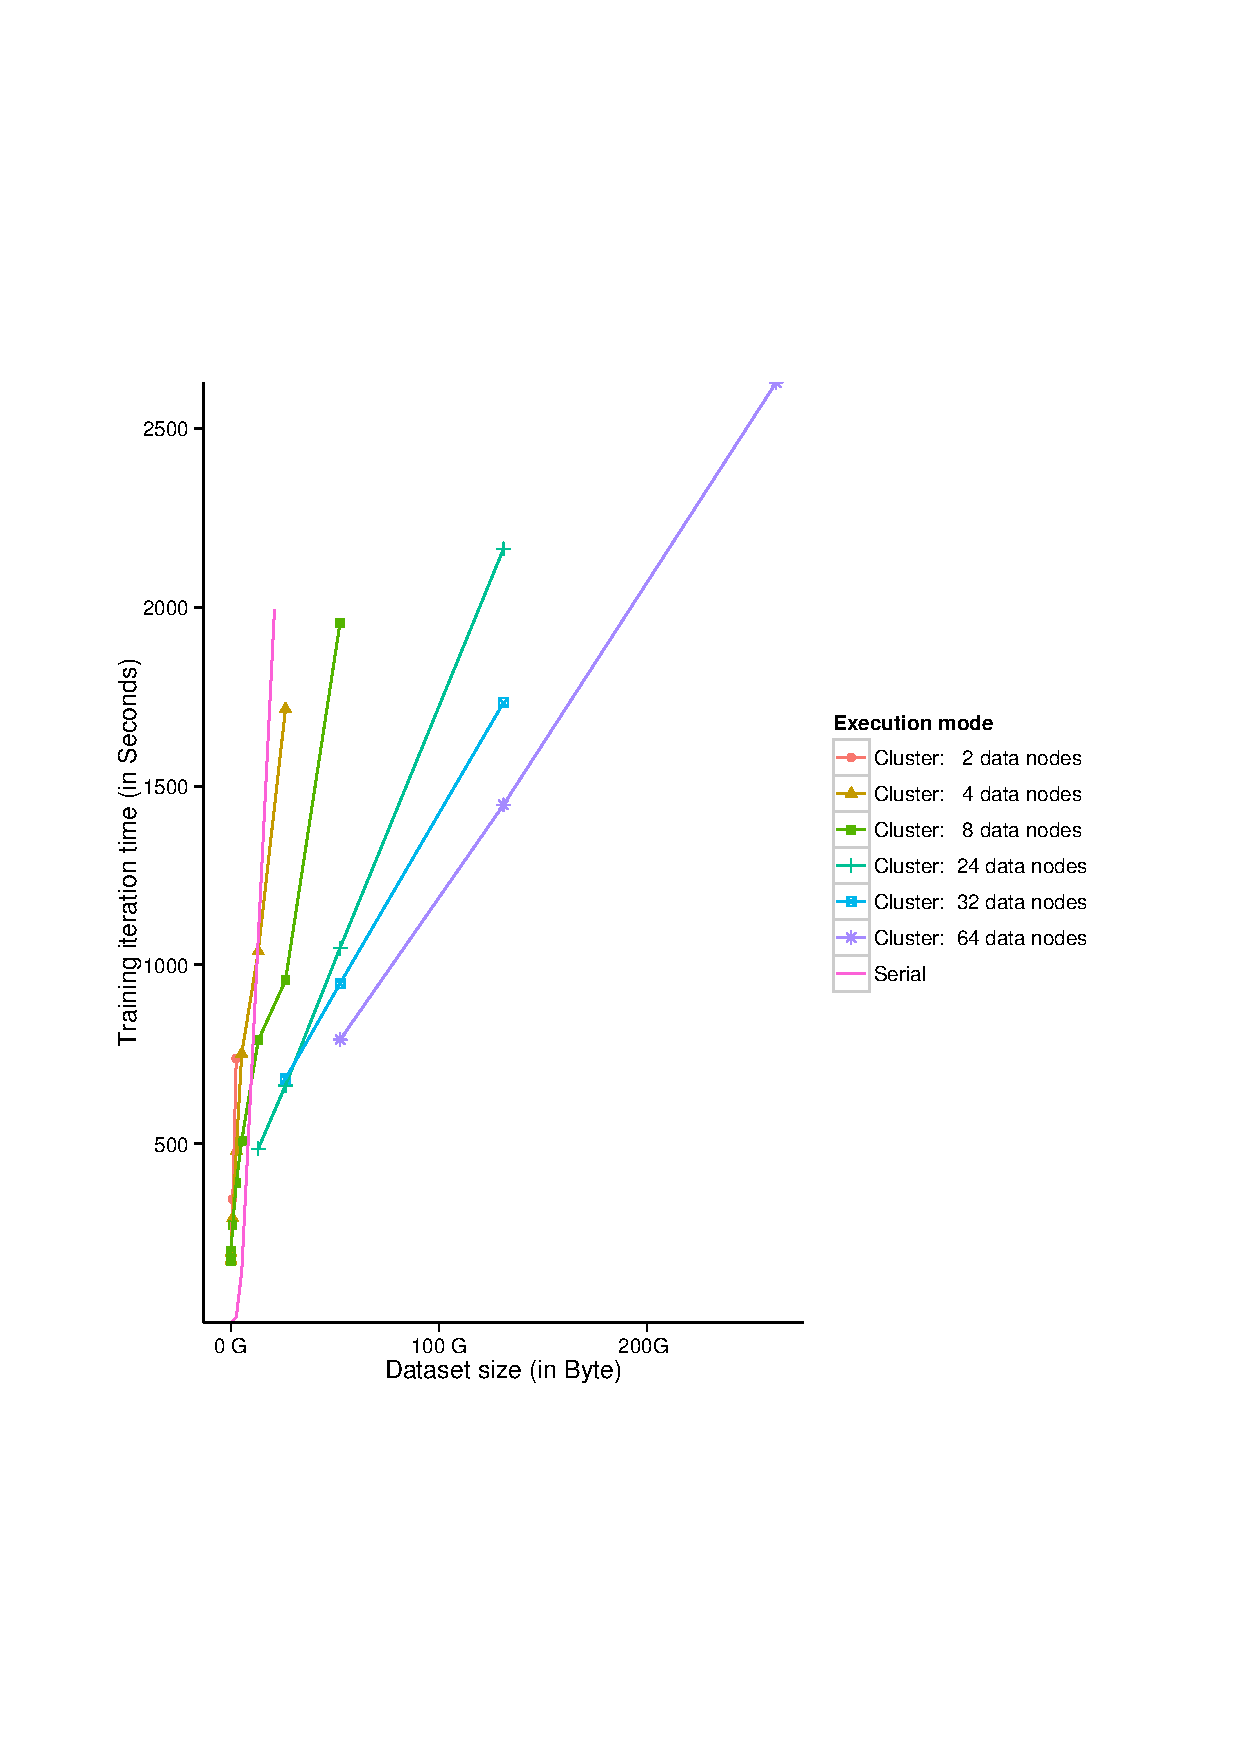
\includegraphics[trim=0cm 5cm 0cm 5cm, scale=0.8]{gfx/time_single.pdf}
\caption{Processing time of a single ListNet training iteration}
\label{fig:listnet_train_time}
\end{figure}

\begin{figure}
\centering
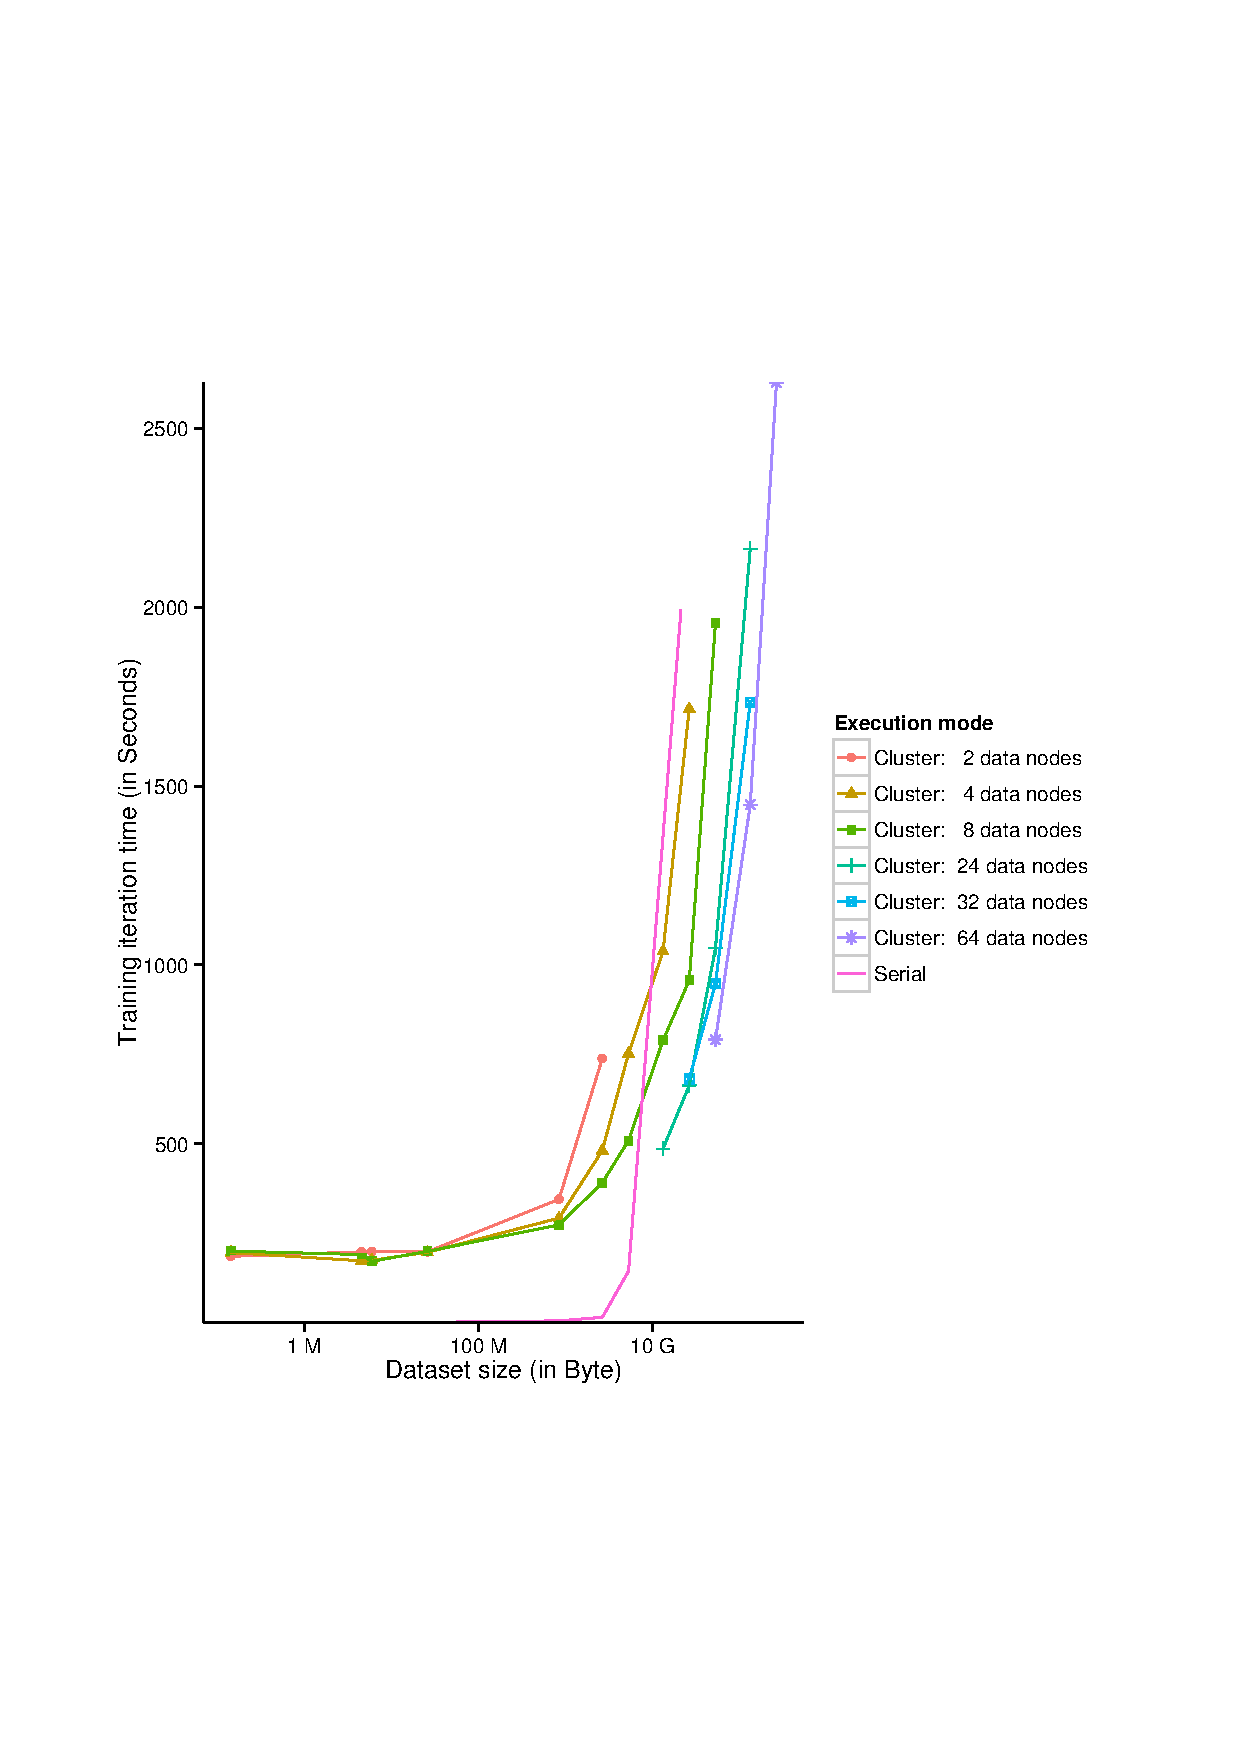
\includegraphics[trim=0cm 5cm 0cm 5cm, scale=0.8]{gfx/time_single_logx.pdf}
\caption{Processing time of a single ListNet training iteration on a logarithmic data size axis}
\label{fig:listnet_train_time_log}
\end{figure}

Figure \ref{fig:speedup_train_time} shows that the speed-up achieved as function of the number of processing data nodes is sub-linear, from which we can deduct that the training time converges to a constant unit of time. Based on our measurements on the small data sets MINI, OHSUMED, MQ2008 and MQ2007, this constant time seems to be within the range of 150 to 200 seconds. This time is likely to be caused by Hadoop job scheduling overhead, this presumption is strengthened by long waiting periods between the separate MapReduce jobs that form a training iteration.\\

Amdahl's law states that the speed-up of a program using parallel computing is limited by the time needed for the sequential fraction of the program. A consequence of Amdahl's Law is that all parallel programs that have a non-parallelisable part have sub-linear speed-up. Behaviour in accordance with Amdahl's law can be seen in Figure \ref{fig:speedup_train_time}, where the speed-up is sub-linear as a result of the existence a non-parallelisable fraction of the program.\\

Note however that Hadoop job scheduling overhead is independent of data set size. Therefore, the non-parallelisable fraction of the program will be smaller when the to be processed data set is larger, allowing larger speed-up values for larger data sets. From this observation we can derive that for \emph{"large enough"} data sets, the speed-up obtained by parallelising ListNet using Hadoop MapReduce is large enough for the parallelisation to be beneficial in terms of processing time compared to the RankLib single-machine version of ListNet, even when the size of the to be processed data set would not have been memory-bounded in RankLib ListNet.\\

Figure \ref{fig:listnet_processing_speed} shows the processing speed in bytes per second. Our observation that RankLib ListNet performs very slow for data sets that do not fit in physical memory and virtual memory is needed is very notable in this graph. Furthermore, this graph shows how both increase in number in data nodes in a cluster and increase in input data size result in an increase in processing speed. The sub-linear growth of processing speed as a factor of input data size can again be explained as a result of the non-parallelisable Hadoop job scheduling part of the operation.\\

A result of that the Hadoop job scheduling overhead does not grow when the input data grows, is that the speed-up is linear or potentially better than linear as a function of data size. This can be seen in Figure \ref{fig:listnet_train_time}. In this Figure the cluster run lines are linear or, in case of the 24 and 32 data nodes cluster lines, slightly better than linear. The lines of the clusters of 8 data nodes or smaller have high variance, this can be attributed to the fact that these clusters were mostly tested on very small datasets, leaving the measurement very dependent on the variance of the job scheduling overhead.

\begin{figure}
\centering
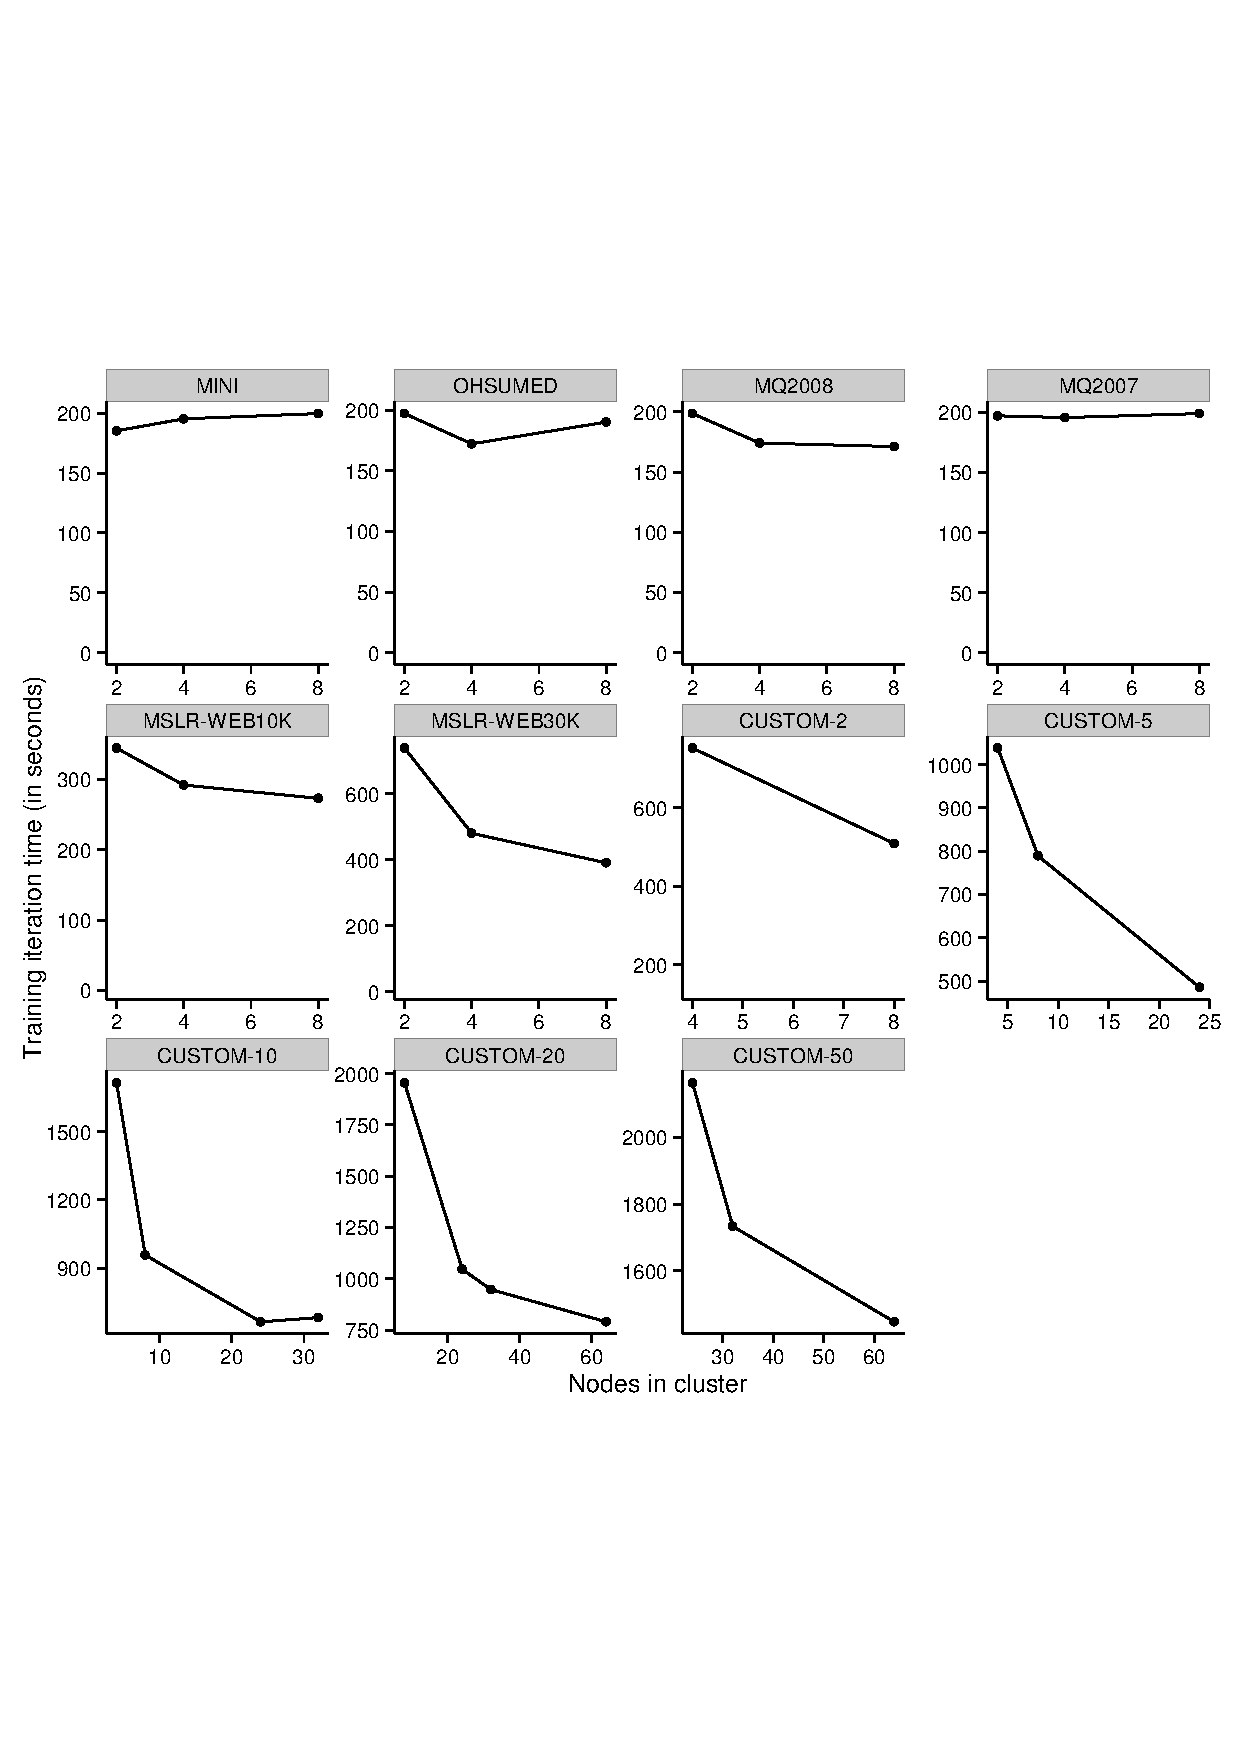
\includegraphics[trim=0cm 5cm 0cm 5cm, scale=0.7]{gfx/speedup_faceted.pdf}
\caption{Processing time of a single ListNet training iteration as a function of the number of data nodes in a cluster}
\label{fig:speedup_train_time}
\end{figure}

\begin{figure}
\centering
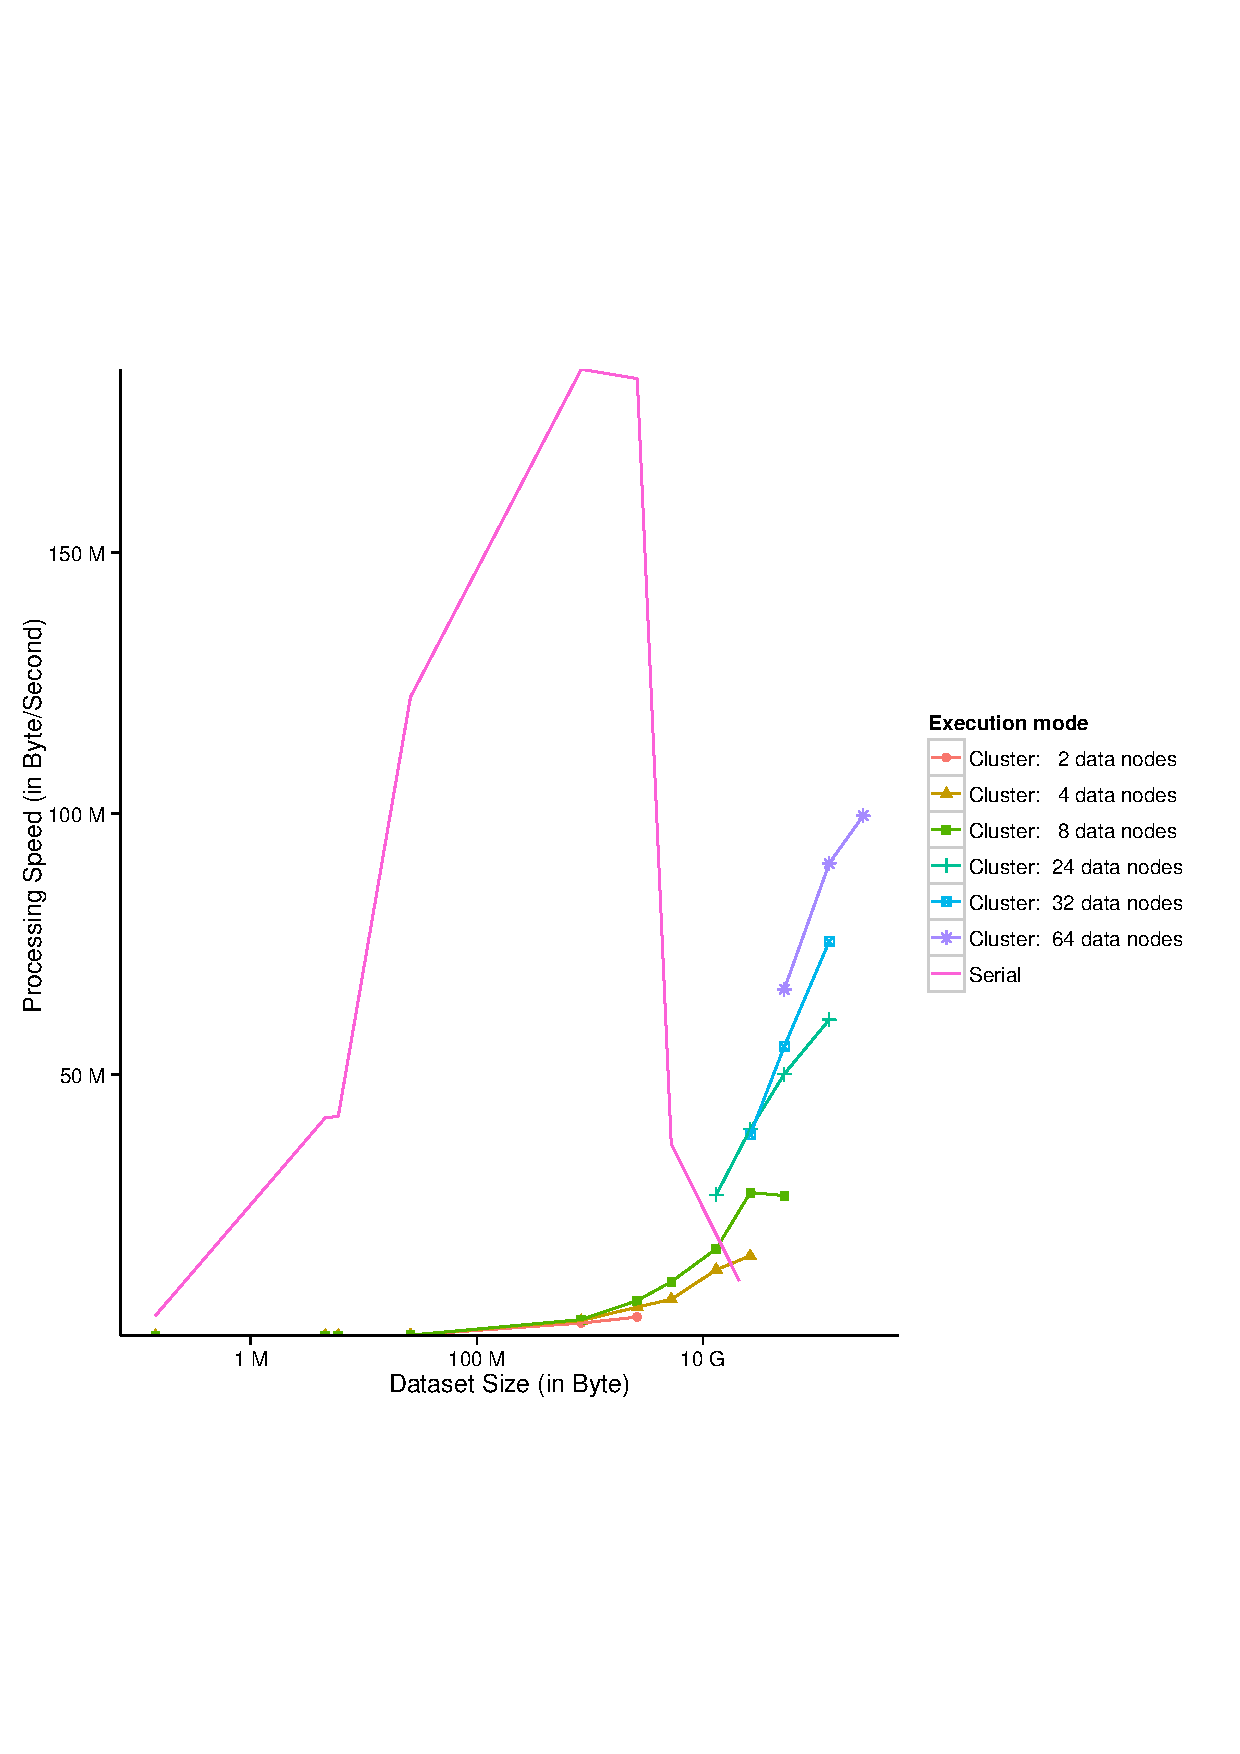
\includegraphics[trim=0cm 5cm 0cm 5cm, scale=0.8]{gfx/processing_speed_single_logx.pdf}
\caption{Processing speed of a a single ListNet training iteration on various data sets}
\label{fig:listnet_processing_speed}
\end{figure}

\section{SmoothRank}